\section{Data Preparation} 
Our data are collected from the website of China Judgements Online. The Chinese government has been publishing the judgement documents on it since 2013\footnote{There are also judgements before 2013.}. We randomly choose 50,000 judgements as training data, 5,000 for validation and 5,000 for test. To ensure enough training data for each charge, we only keep the charges that appear more than 50 times in the training data. As for law articles, we only consider the ones in Chinese Criminal Law. The resulting dataset contains 50 distinct charges and 321 distinct articles. About 3.56\% cases contain more than one charges, and 94.18\% cases contain more than one law articles. \orange{An average case has 1.03 charges and 3.81 law articles}. The fact description part of each judgement document contains 382.60 words, and 14.21 sentences on average.

\begin{figure*}[t!]
\begin{center}
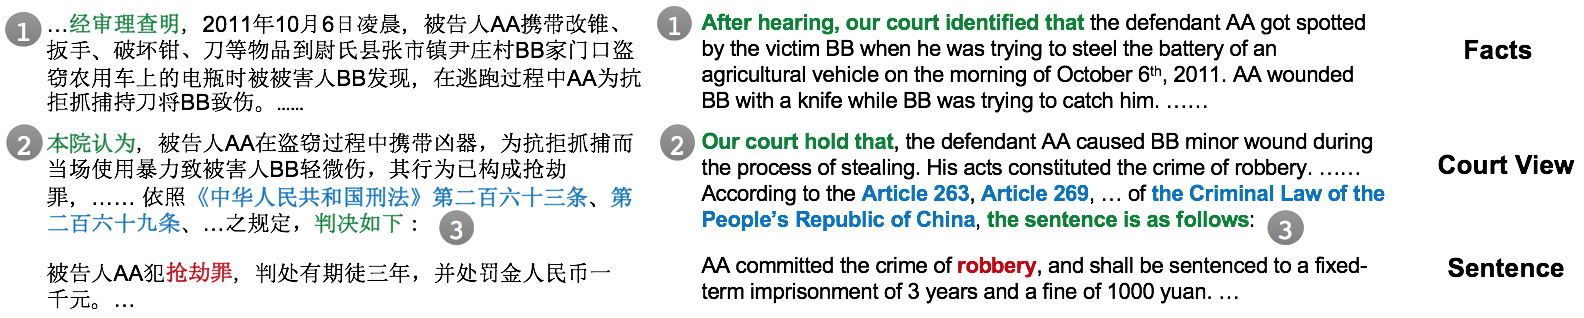
\includegraphics[width=0.97\textwidth]{figures/case.png}	
\caption{Example Judgement Document of a Chinese Criminal Case}
\label{fig_example_case}
\end{center}
\end{figure*}

An example judgement is shown in Figure \ref{fig_example_case}. Although there does not exist a strict rule for formatting a judgement document, we can still discover some patterns in it. A typical judgement document often starts with a brief description of the \emph{procedure} \orange{followed before the judgement}, from the start of the prosecution until the case is decided. The procedure part is often followed by the \emph{facts} of the case. After that, the court will conclude the case and provide relevant law articles that can be applied to the case (\emph{court view}). Finally, the \emph{sentence} part will list the charges of the defendant along with the corresponding penalties. 

We find that the fact description part often starts with the clause 经审理查明$\ $(after hearing, our court identified that), the court view part often starts with the clause 本院认为$\ $(our court hold that), and the sentence part often starts with the clause 判决如下$\ $(\orange{the sentence is as follows}). Therefore we extract the texts between these two clauses as fact description, and consider the text after 判决如下$\ $as sentence part. Since the charge mentions do not have many variations in judgement documents, we manually build a list that contains the possible variations of each charge based on a public criminal charge list\footnote{\url{http://china.findlaw.cn/zuiming/}}. The resulting list is used to find charge mentions in the sentence part with exact matching. As for law articles, since the article is often mentioned in a fixed patterns, we simply use a regular expression\footnote{``第[、零〇一二两三四五六七八九十百千0-9]+条(之[一二两三四五六七八九十])?)''} to identify the article mentions. 

Note that we only retain the cases with one defendant. Because in the situation with multiple defendants, it is hard to separately relate each defendant to his (or her) corresponding facts, articles and charges due to the unstructured nature of the judgement document.